\chapter{Lecture 6 - Newton's Method for Systems of Non-Linear Equations}
\label{ch:lec6n}
\section{Objectives}
The objectives of this lecture are to:
\begin{itemize}
\item Describe Newton's method for finding roots to systems of non-linear equations.
\item Do an example problem.
\item Describe MATLAB functions for solving a system of non-linear equations.
\end{itemize}
\setcounter{lstannotation}{0}

\section{Newton's Method for Systems of Non-Linear Equations}

In Lecture 4 we derived Newton's method for finding the root to a single non-linear equation.  The basic iteration procedure was to update our estimate of the root according to the equation:
\begin{equation*}
x_{i+1} = x_i - \frac{f(x_i)}{f^{\prime}(x_i)}
\end{equation*}
The idea on which this was derived was to project a line tangent to $f(x_i)$ to the $x$-axis. 

\index{Taylor series expansion}
\newthought{An alternative way} to derive this update relation is based on the Taylor series expansion.  In a Taylor series expansion, given a function evaluated at some point, $f(x_1)$, we estimate the value of the function at some \emph{other} point, $x_2$, using the equation below:

\begin{align*}
f(x_2) &= f(x_1) +  \frac{f^{\prime}(x_1)}{1!}(x_2 - x_1) +  \frac{f^{\prime \prime}(x_1)}{2!}(x_2 - x_1)^2 + \cdots \\
&= \sum\limits_{n=0}^{\infty} \frac{f^{(n)}(x_1)}{n!}(x_2 - x_1)^n
\end{align*}
If we ignore terms proportional to $f^{\prime \prime}(x_1)$ and higher, and if we suppose that $x_2$ is a root, we get:
\begin{align*}
f(x_2) = 0 &= f(x_1) + f^{\prime}(x_1)(x_2 - x_1) \\
x_2 - x_1 &= \frac{-f(x_1)}{f^{\prime}(x_1)} \\
\Rightarrow x_2 &= x_1 - \frac{f(x_1)}{f^{\prime}(x_1)} 
\end{align*}
which is the same as what we started with.

\newthought{We would now} like to generalize Newton's method to find roots for a \emph{system} of two or more equations.  We will use the formulation based on the Taylor series expansion to do this.  

Consider the case of 2 non-linear functions of 2 variables:
\begin{equation*}
f_1(x,y) = 0 , \ \ f_2(x,y) = 0
\end{equation*}
If $x_2$ and $y_2$ are the true (unknown) solution to the equations, and $x_1$ and $y_1$ are points sufficiently close to the solution then:
\begin{align*}
f_1(x_2,y_2) &= 0 = f_1(x_1,y_1) + (x_2 - x_1) \frac{\partial f_1}{\partial x}\Bigr|_{x_1,y_1} + (y_2 - y_1) \frac{\partial f_1}{\partial y}\Bigr|_{x_1,y_1}  \\
f_2(x_2,y_2) &= 0 = f_2(x_1,y_1) + \underbrace{(x_2 - x_1)}_{\Delta x} \frac{\partial f_2}{\partial x}\Bigr|_{x_1,y_1} + \underbrace{(y_2 - y_1)}_{\Delta y} \frac{\partial f_2}{\partial y}\Bigr|_{x_1,y_1} \\
\end{align*}
where higher order terms are neglected.  This set of linear equations can be expressed in a matrix-vector format as shown in Equation \ref{eq:lec6n-matvec}.

\index{Jacobian}
\begin{equation}
\bracketMatrixstack{
\frac{\partial f_1}{\partial x}\Bigr|_{x_1,y_1} & \frac{\partial f_1}{\partial y}\Bigr|_{x_1,y_1} \\
\frac{\partial f_2}{\partial x}\Bigr|_{x_1,y_1} & \frac{\partial f_2}{\partial y}\Bigr|_{x_1,y_1}
}
\bracketVectorstack{
\Delta x \\
\Delta y
}
=
\bracketVectorstack{
-f_1(x_1,y_1) \\
-f_2(x_1,y_1)
}
\label{eq:lec6n-matvec}
\end{equation}
The unknown quantities are $\Delta x$ and $\Delta y$.  The matrix in Equation \ref{eq:lec6n-matvec} is referred to as the \emph{Jacobian}. We can solve this linear system of equations\sidenote{Actually we have not covered how to do that yet in this class.  Students can probably solve this $2 \times 2$ system of equations based on their experience in high school math, but we will thoroughly study methods for solving linear systems of equations in the next section of the text.} to find $\Delta x$ and $\Delta y$ and thus get $x_2$ and $y_2$ from Equation \ref{eq:lec6n-xy-update}.
\begin{equation}
x_2 = x_1 + \Delta x, \ \ \ y_2 = y_1 + \Delta y
\label{eq:lec6n-xy-update}
\end{equation}

\vspace{4.0cm}

\newthought{In summary,} Newton's method for solving a system of non-linear equations is made up of the following steps:
\begin{enumerate}
\item Start with an initial guess, $x_1$, $y_1$.
\item Form and solve the linear system of equations given in Equation \ref{eq:lec6n-matvec} to obtain $\Delta x$ and $\Delta y$.
\item compute $x_{i+1}$ and $y_{i+1}$ from: $x_{i+1} = x_{i} + \Delta x, $ and $ y_{i+1} = y_{i} + \Delta y$.
\item Repeat steps \#2 and \#3 until $\Delta x$ and $\Delta y$ are within some specified error tolerance.\sidenote{We will use a relative error tolerance that will be illustrated in the example code.}
\end{enumerate}

\vspace{0.25cm}

\noindent\textbf{Example:} The equations of the catenary curve and the ellipse, which are shown in Figure \ref{fig:lec6n-ex1}, are given by:
\begin{marginfigure}
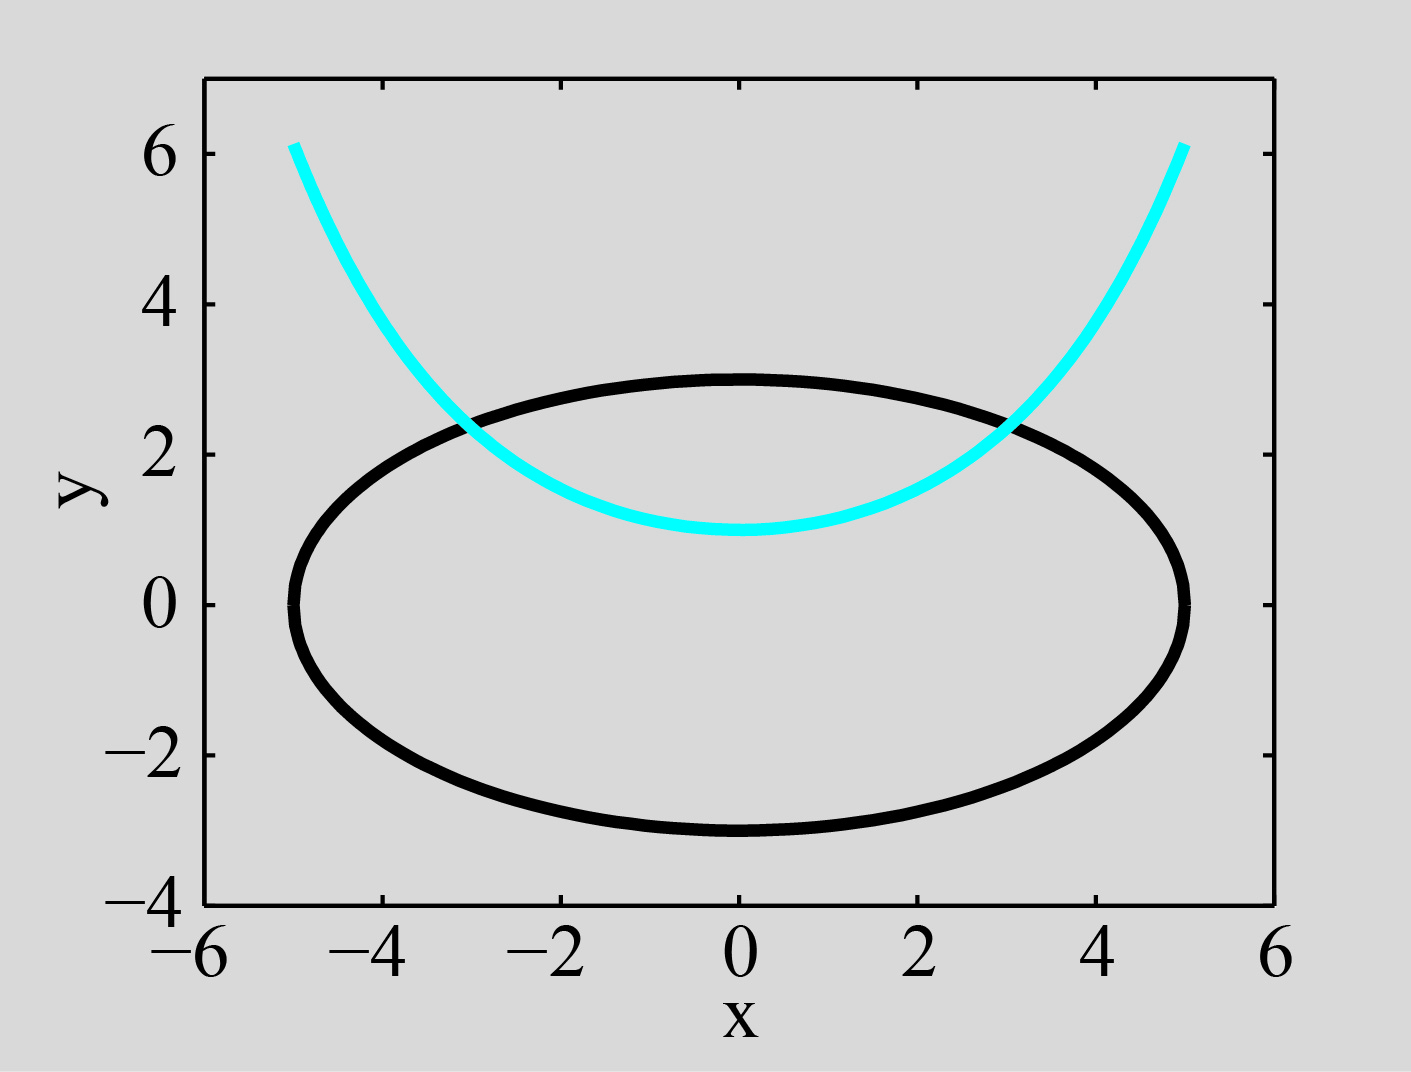
\includegraphics{Chapter3Example3_5.jpg}
\caption{Example system of non-linear equations.}
\label{fig:lec6n-ex1}
\end{marginfigure}
\begin{align*}
f_1(x,y) &= y-\frac{1}{2}\left(e^{\sfrac{x}{2}} + e^{-\sfrac{x}{2}}\right) \\
f_2(x,y) &= 9x^2 + 25y^2 - 225
\end{align*}
Use Newton's method to determine the point of intersection of the curves that resides in the first quadrant of the coordinate system.

\vspace{0.15cm}

\noindent The Jacobian for this system of equations is given by:
\begin{equation*}
\bracketMatrixstack{
-\frac{1}{4}\left(e^{\sfrac{x}{2}} + e^{-\sfrac{x}{2}}\right) & 1 \\
18x & 50y 
}
\end{equation*}

\vspace{0.15cm}

\noindent We begin by clearing out the workspace and defining the given functions and the Jacobian:
\begin{lstlisting}[style=myMatlab, name=lec6n-ex1]
clear
clc
close 'all'

F1 = @(x,y) y - 0.5*(exp(x./2) + exp(-x./2));
F2 = @(x,y) 9*x.^2 + 25*y.^2 - 225;

dF1x = @(x,y) -0.25*(exp(x./2) - exp(-x./2));
dF1y = @(x,y) 1;

dF2x = @(x,y) 18*x;
dF2y = @(x,y) 50*y;

Jac = @(x,y) [dF1x(x,y) dF1y(x,y); dF2x(x,y) dF2y(x,y)];
\end{lstlisting}

\vspace{0.15cm}

\noindent Next we will define $x_1$ and $y_1$ and specify our stopping criteria.
\begin{lstlisting}[style=myMatlab,name=lec6n-ex1]
xi = 2.5; yi = 2; 
Err = 1e-10; imax = 10;
\end{lstlisting}
Note that we do not plan on making many iterations.  If Newton's method works, it will very quickly converge.

\vspace{0.25cm}

\noindent Now we implement Newton's method:\marginnote[1.0cm]{
\ref{lst:ann6n-1} We use MATLAB's built-in ``backslash'' operator to solve the linear system of equations.  This will be discussed in Section VIII of this text.

\vspace{0.3cm}


\ref{lst:ann6n-2} Here we compare $\sfrac{\Delta x}{x}$ and $\sfrac{\Delta y}{y}$ for our relative error tolerance.  We are really not computing the error, we are computing how small our updates are to $x$ and $y$.

\vspace{0.5cm}

\ref{lst:ann6n-3} The operator \lstinline[style=myMatlab]{&&} is the logical \emph{and} operator.

}
\begin{lstlisting}[style=myMatlab,name=lec6n-ex1]
for i = 1:imax
   J = Jac(xi,yi);
   F = -[F1(xi,yi); F2(xi,yi)];
   dp = J\F;   /*!\annotation{lst:ann6n-1}!*/
   xip = xi + dp(1);
   yip = yi + dp(2);
   Err_x = abs((xip - xi)/xi);  /*!\annotation{lst:ann6n-2}!*/
   Err_y = abs((yip - yi)/yi);
   
   fprintf('i = %i  x = %-7.4f  y = %-7.4f  Error in x = %-7.4g Error in y = %-7.4g \n',...
       i,xip,yip,Err_x,Err_y);
   
   if (Err_x < Err) && (Err_y < Err)  /*!\annotation{lst:ann6n-3}!*/
       break
   else
       xi = xip; yi = yip;
   end
    
end
\end{lstlisting}
This script converges to the solution $x = 3.0311553917$ and $y=2.38586565356$ in 5 iterations.

\section{Implementation with FSOLVE}
The primary MATLAB built-in function you should use for solving a system of non-linear equations is \lstinline[style=myMatlab]{fsolve}.  The basic syntax for using \lstinline[style=myMatlab]{fsolve} is:
\begin{center}
\begin{tabular}{c}
\begin{lstlisting}[style=myMatlab, frame=none, numbers=none, basicstyle=\small]
x = fsolve(fun,x0);
\end{lstlisting}
\end{tabular}
\end{center}
A more complete syntax that provides additional output information and an interface for passing options to the algorithm is:
\begin{center}
\begin{tabular}{c}
\begin{lstlisting}[style=myMatlab, frame=none, numbers=none, basicstyle=\small]
[x, fval, exitflag, output, jacobian] = ...
     fsolve(fun,x0,options);
\end{lstlisting}
\end{tabular}
\end{center}
The values of \lstinline[style=myMatlab]{x} and \lstinline[style=myMatlab]{fval} are similar to what one obtains when using \lstinline[style=myMatlab]{fzero} except, of course they are now both vectors.  Values for \lstinline[style=myMatlab]{exitflag} and \lstinline[style=myMatlab]{output} are different---interested readers should consult the MATLAB documentation---but \lstinline[style=myMatlab]{exitflag=1} still means success.  As with \lstinline[style=myMatlab]{fzero}, a function is used to construct an appropriate \lstinline[style=myMatlab]{options} structure; when using \lstinline[style=myMatlab]{fsolve} you should use the \lstinline[style=myMatlab]{optimoptions} function for this purpose. An example usage of \lstinline[style=myMatlab]{optimoptions} is included in the MATLAB listing below.

\vspace{3.0cm}

\marginnote[4.0cm]{

\ref{lst:ann6n-1} Here we use a \lstinline[style=myMatlab]{switch...case} structure to select between sets of options for purposes of demonstration. The options specified in \lstinline[style=myMatlab]{option_set=1} amount to telling \lstinline[style=myMatlab]{fsolve()} to quietly solve the problem with no output to the command window.  The options specified in \lstinline[style=myMatlab]{option_set=2} specify detailed output on each iteration and provides non-default values for the \lstinline[style=myMatlab]{'MaxIterations'} and \lstinline[style=myMatlab]{'StepTolerance'} parameters.  Consult the MATLAB documentation on \lstinline[style=myMatlab]{fsolve} for more details.

\vspace{3.5cm} 

\ref{lst:ann6n-2} The first argument to \lstinline[style=myMatlab]{fsolve} has to be a (single) handle to a function.  This local function implements the system of two equations from the example. The first argument to \lstinline[style=myMatlab]{ex3p5} is a vector; one element for each equation in our system of equations.

}
\begin{lstlisting}[name=lec6n-ex2, style=myMatlab]
clear
clc
close 'all'

F = @(x) ex3p5(x);
X0 = [2.5, 2.0];

option_set = 2;
% 1 = no outputs
% 2 = detailed outputs

switch option_set     /*!\annotation{lst:ann6n-1}!*/
    
    case 1
        options = optimoptions('fsolve','Display','none');
        
    case 2
        options = optimoptions('fsolve','Display',...
            'iter-detailed','MaxIterations',1000,...
            'StepTolerance',1e-10);
        
    otherwise % default options
        options = optimoptions('fsolve');
        
end

[x,fval,exitflag,output] = fsolve(F,X0,options);

fprintf('Root found at x = %8.7g, y = %8.7g \n',...
    x(1),x(2));
fprintf('fval = \n'); disp(fval);
fprintf('exitflag = %d \n',exitflag);

%% Local Function
function out = ex3p5(x)   /*!\annotation{lst:ann6n-2}!*/
[m,n] = size(x); % expect scalar or vector input
assert(min(m,n)==1,...
    'Error!  Vector input expected for x! \n');
out = nan(m,n); % construct output

out(1) = x(2) - 0.5*(exp(x(1)./2) + exp(-x(1)./2));
out(2) = 9*x(1).^2 + 25*x(2).^2 - 225;

end
\end{lstlisting}
  

